\documentclass{article}

% for source code listings
\usepackage{listings}
\lstset{language=Python,
	showstringspaces=false}

% smaller margins
\usepackage{anysize}
\marginsize{3cm}{2cm}{1cm}{1cm}

% for figures
\usepackage[pdftex]{graphicx}

% use colorlinks option instead of default 'ugly box' link highlighting
\usepackage{url}
\usepackage[colorlinks]{hyperref}

% to monospace things
\newcommand{\mono}[1]{\texttt{#1}}

% macros for monospaced package names, etc
\newcommand{\cmepy}{\mono{CmePy}}
\newcommand{\python}{\mono{Python}}
\newcommand{\numpy}{\mono{NumPy}}
\newcommand{\scipy}{\mono{SciPy}}
\newcommand{\pylab}{\mono{PyLab}}
\newcommand{\matplotlib}{\mono{matplotlib}}

% for inline python code snippets
\newcommand{\code}[1]{\lstinline$#1$}

% to refer to listings
\newcommand{\lstref}[1]{Listing~\ref{#1}}

% to refer to figures
\newcommand{\figref}[1]{Figure~\ref{#1}}

% for mailto links
\newcommand{\mailto}[1]{\href{mailto: #1}{#1}}

\title{A \cmepy{} Tutorial}
\author{Reuben Fletcher-Costin}

\begin{document}

\maketitle

\tableofcontents

\section{Overview}

\cmepy{} is a \python{} package to assist in the numerical solution of the
Chemical Master Equation (CME).

\section{Installation}

\subsection{Dependencies}
\cmepy{} was developed with \python{} 2.5.2, \scipy{} 0.7.0, \& \numpy{} 1.2.1 .
In addition, \matplotlib{} is used to display graphical output in some
examples, but is not otherwise a dependency.

\subsection{Testing \& Installation}

Once \cmepy{} has been obtained, the package can be tested and installed
by running the \mono{setup.py} script via \python{} as follows:

\mono{python setup.py test}

\mono{python setup.py install}

\subsubsection{Local package installation (Linux)}
If it is not possible to install \cmepy{} to the \python{}'s global
\mono{site-packages} directory, \cmepy{} may be installed locally to a user's
\mono{\$\{HOME\}} directory. First, ensure the path
\mono{\$\{HOME\}/lib/python} exists,
and that the \mono{\$\{PYTHONPATH\}}
environment variable includes
\mono{\$\{HOME\}/lib/python}. Then, \cmepy{} may be installed locally via

\mono{python setup.py install --home=\$\{HOME\}}

A (possibly better) alternative to this method of local installation is to
use the \mono{virtualenv} package to establish isolated (local)
\python{} environments. See \url{http://pypi.python.org/pypi/virtualenv}.

\section{Examples}

\subsection{Basic \mono{CmeSolver} usage}

We begin with a simple example illustrating the basic usage of \cmepy{}'s
\mono{CmeSolver} class. The code for this example is shown below in
\lstref{basicSolverUsage}.

\begin{lstlisting}[frame=tb,
caption={Example: solving a model},
label=basicSolverUsage
]
import numpy
from cmepy.solver import CmeSolver
from cmepy.models import MM_simple as model

solver = CmeSolver(model)

time_steps = numpy.linspace(0, 2.5, 51)
for t in time_steps:
    solver.step(t)

solution = solver.get_p()
\end{lstlisting}

In this first example, we load \mono{MM\_simple}, one of the pre-defined models
supplied with \cmepy{}. This model is for a simple Michaelis-Menten system,
consisting of three reactions. The model definition format will be explained
later, in subsection~\ref{subsectionModels}.

After loading the model for the Michaelis-Menten system under the name
\mono{model}, we create a \mono{CmeSolver} instance for this model, then step
the solver forward, advancing the solution of the chemical master equation,
from time $t = 0.0$ to time $t = 2.5$ seconds. Finally, we extract $p$, the
(reaction-count) probability distribution for $t = 2.5$, and store it under the
name \mono{solution}. Since the system we are modelling has three reactions,
the resulting probability distribution returned by \mono{solver.get\_p()} is a
three-dimensional \numpy{} array.

\subsection{Combining \mono{CmeSolver}, \mono{CmeRecorder} \& \pylab{} for
graphical output}

We can extend the previous example to record and plot the expected species
counts. \cmepy{} includes a convenience class, \mono{CmeRecorder}, which is
able to compute and store a number of common measurements. In this example,
shown in \lstref{combiningSolverRecorderPylab}, we use \mono{CmeRecorder} to
compute the expected count of each species in the system, at each time step,
and then plot these measurements using \pylab{}. The resulting plot is
displayed in \figref{fig:combiningSolverRecorderPylab}

\begin{lstlisting}[frame=tb,
caption={Example: solving a model and plotting species counts},
label=combiningSolverRecorderPylab]
import numpy
import pylab
from cmepy.solver import CmeSolver
from cmepy.recorder import CmeRecorder
from cmepy.models import MM_simple as model

solver = CmeSolver(model)

recorder = CmeRecorder(solver)
recorder.add_target(output = ['expectation'],
                    species = model['species'])

time_steps = numpy.linspace(0, 2.5, 51)
for t in time_steps:
    solver.step(t)
    recorder.take_measurements()

pylab.figure()
for s_info in recorder.measurements('species'):
    pylab.plot(s_info.times,
               s_info.expectation,
               label = s_info.name)
pylab.legend()
pylab.title('Expectation values of species counts')
pylab.show()
\end{lstlisting}

\begin{figure}[p!]
\centering
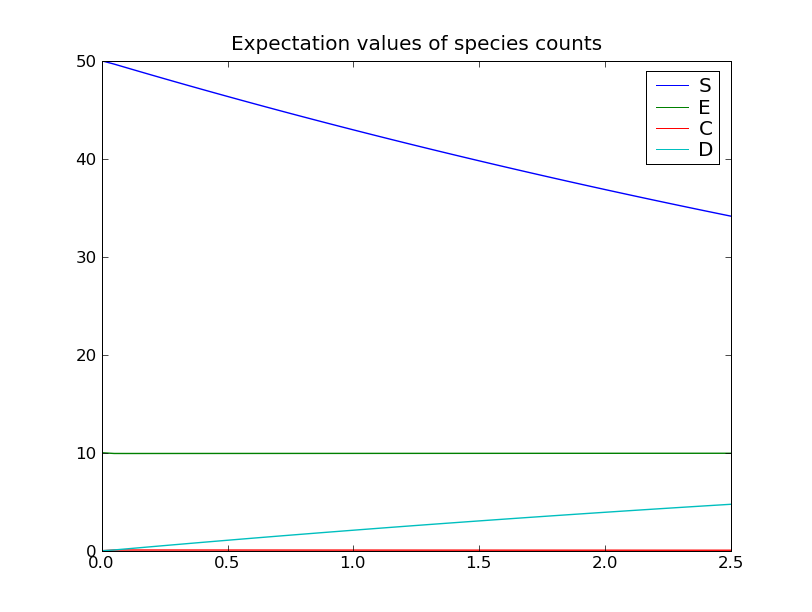
\includegraphics[width=0.5\textwidth]{./fig_combiningSolverRecorderPylab.png}
\caption{Output produced by \lstref{combiningSolverRecorderPylab}.}
\label{fig:combiningSolverRecorderPylab}
\end{figure}

\subsection{Setting \mono{CmeSolver} initial conditions}
By default, when a \mono{CmeSolver} instance is initialised for a model, default
values for the initial time $t_0$ and initial probability distribution $p_0$
are used. The default initial time is $0$, while the default initial
probability distribution is probability $1$ at the origin of the reaction
count state space -- that is, the state where all reaction counts are zero --
and probability $0$ for all other states.

However, it is possible to explicitly pass initial conditions to the solver,
by calling the method \mono{set\_initial\_values(t0, p0)}. Here, \mono{t0}
specifies the time of the initial probability distribution, while \mono{p0}
specified the initial probability distribution. \mono{p0} must be a \numpy{}
array, of the shape \mono{model['np']}. Since \mono{p0}
is a probability distribution, all elements of the array should be non-negative,
and sum to unity, although these are not hard-requirements
\footnote
{
	In fact, due to the nature of the numerical computations, probability
	distributions \emph{returned} by the solver typically contain some
	(very small) non-positive elements.
}
.

An example of specifying custom initial conditions is given below in
\lstref{solverSetInitialValues}.
Here, the initial probability distribution is set to be uniformly zero,
except for the states where the count of the first
reaction is $0$ or $1$, and the count of the second reaction is $0$, where the
probability is set to $0.5$. The initial time is specified to be $10.0$ seconds.

\begin{lstlisting}[frame=tb,
caption={Example: specifying initial conditions},
label=solverSetInitialValues
]
import numpy
from cmepy.solver import CmeSolver
from cmepy.models import A2B2C as model

solver = CmeSolver(model)

#compute & set custom initial conditions for solver
p_0 = numpy.zeros(models['np'])
p_0[0, 0] = 0.5
p_0[1, 0] = 0.5

time_steps = numpy.linspace(10.0, 20.0, 11)
t_0 = time_steps[0]

solver.set_initial_values(t_0, p_0)

#solve the model
for t in time_steps:
	solver.step(t)
\end{lstlisting}

\subsection{Defining new models}
\label{subsectionModels}


%    propensities    : a sequence of propensity functions, mapping reaction
%                      counts to reaction propensities, for each reaction.
%    np              : a sequence of positive integers specifying the
%                      dimensions of the reaction count state space.
%                      In this example, np contains only one element,
%                      indicating that there is only one reaction in the
%                      system, and that the corresponding reaction count
%                      takes 11 possible values: 0, 1, 2, 3, ..., 10 .

It is reasonably straight-forward to define new models.
We will introduce the model format, and some useful techniques, by considering a
sequence of examples.
To begin, we start with a very simple system, consisting of two species, $A$
and $B$, and a single reaction $A \rightarrow B$. We assume that the initial
conditions consist of $10$ copies of the species $A$, and $0$ copies of the
species $B$. A minimal model for this system is defined below in
\lstref{model1a}.

\begin{lstlisting}[frame=tb,
caption={A minimal model definition for the system $A \rightarrow B$.},
label=model1a]
model = {'propensities' : (lambda x : 1.0*(10-x), ),
         'np' : (11, ),
         }
\end{lstlisting}

As can be seen in the example, models are simply defined as
\python{} dictionaries. The minimal
\footnote
{
	Here, we mean \emph{minimal} in the sense that the presence of
	both these fields is both necessary and sufficient
	for this model to be solvable via a
	\mono{cmepy.solver.CmeSolver}
	instance.
}
information a model must supply
are the fields \mono{propensities} and \mono{np}.

The field \mono{propensities}
should be a sequence (i.e. tuple, list, etc.) of propensity functions, one
for each reaction in the system, mapping reaction counts to reaction
propensities.

In this example we have used \python{}'s \mono{lambda}
shorthand to succinctly define the propensity function as an unnamed function,
mapping \mono{x}, the number of times the reaction has occurred, to the
propensity of the reaction, \mono{1.0 * (10-x)}. Observe that if $x$ is the
number of times that the reaction $A \rightarrow B$ has occurred, and that
initially there are $10$ copies of species $A$, then there must currently be $10-x$ copies of
species $A$.

The field \mono{np} is a sequence of positive integers,
specifying the dimensions of the reaction count state space. In this example,
there is only one reaction in the system, hence \mono{np} only contains one
element, and the corresponding reaction count may range over the $11$ possible
values: $0, 1, 2, 3, \ldots, 10$ .

For the second example, we extend the minimal model from \lstref{model1a}
to define a full model for the same system, shown below in \lstref{model1b}.

\begin{lstlisting}[frame=tb,
caption={A full model definition for the system $A \rightarrow B$.},
label=model1b]
model = {'doc' : 'example model for reaction A -> B',
         'propensities' : (lambda x : 1.0*(10-x), ),
         'reactions' : ('A->B', ),
         'species counts' : (lambda x : 10-x,
                             lambda x : x, ),
         'species' : ('A', 'B', ),
         'np' : (11, ),
         }
\end{lstlisting}

The \mono{propensities} and \mono{np} fields remain unchanged, but there are
a number of additional fields:
\begin{itemize}
  \item \mono{doc} : a brief description of the model;
  \item \mono{reactions} : a sequence of reaction names, using the same
  ordering as the sequence of propensity functions;
  \item \mono{species counts} : a sequence of functions, each mapping
  reaction counts to a species count, for each species in the model
  \item \mono{species} : a sequence of species names, using the same ordering
  as the sequence of species count functions.
\end{itemize}

While a system consisting of only a single reaction is a good introduction
to the model format, most systems of interest will feature two or more
reactions.
For the next example, we shall consider a system of two reactions,
defined below in \lstref{model2a}.

 \begin{lstlisting}[frame=tb,
caption={A minimal model definition for the system
$A \rightarrow B$, $B \rightarrow C$.},
label=model2a]
model = {'propensities' : (lambda x1, x2 : 1.0*(10-x1),
                           lambda x1, x2 : 1.0*(x1-x2),),
         'np' : (11, 11, ),
         }
\end{lstlisting}

As the system consists of two reactions, both the \mono{propensities} and
\mono{np} fields now contain two elements. Observe that each propensity function
must now take two arguments, \mono{x1} and \mono{x2}, which are the reaction counts
of the first and second reactions respectively. Apart from the addition
of a second unused argument, the first propensity function has the same form
as that defined in the first example, \lstref{model1a}.

Note, in the second propensity function, that the difference \mono{x1 - x2} is
the count of reaction $A \rightarrow B$ minus the count of reaction
$B \rightarrow C$, so this yields the number of copies of the species $B$.

As before, we may expand this minimal two-reaction model into a full model,
as shown in \lstref{model2b}.

\begin{lstlisting}[frame=tb,
caption={A full model definition for the system
$A \rightarrow B$, $B \rightarrow C$.},
label=model2b]
model = {'doc' : 'example model for reactions A -> B, B -> C',
         'propensities' : (lambda x1, x2 : 1.0*(10-x1),
                           lambda x1, x2 : 1.0*(x1-x2), ),
         'reactions' : ('A->B', 'B->C', ),
         'species counts' : (lambda x1, x2 : 10-x1,
                             lambda x1, x2 : x1-x2,
                             lambda x1, x2 : x2, ),
         'species' : ('A', 'B', 'C', ),
         'np' : (11, 11, ),
         }
\end{lstlisting}

For a final example, illustrating some useful techniques, consider the model
below in \lstref{model2c}.

\begin{lstlisting}[frame=tb,
caption={Automatic generation of models for the sustem
$A \rightarrow B$, $B \rightarrow C$, using specified
initial copy counts of the species $A$, $B$ and $C$.},
label=model2c]
def generate_model(initial_count_a,
                   initial_count_b,
                   initial_count_c):
    """
    Generates and returns a complete model for the system of reactions
    A->B, B->C, using the specified initial counts of A, B & C.
    """
    
    # define maps from reaction counts to species counts first
    species_counts = (lambda *x : initial_count_a - x[0],
                      lambda *x : initial_count_b + x[0] - x[1],
                      lambda *x : initial_count_c + x[1], )
    
    # then define the reaction propensities in terms of the species counts
    propensities = (lambda *x : 1.0*species_counts[0](*x),
                    lambda *x : 1.0*species_counts[1](*x), )
    
    model = {'doc' : 'example model for reactions A -> B, B -> C',
             'propensities' : propensities,
             'reactions' : ('A->B', 'B->C', ),
             'species counts' : species_counts,
             'species' : ('A', 'B', 'C', ),
             'np' : (initial_count_a + 1,
                     initial_count_a + initial_count_b + 1, ),
             }
    
    return model

model = generate_model(10, 0, 0)
\end{lstlisting}

\lstref{model2c} is a re-formulation of the same model from
\lstref{model2b}, employing a number of techniques:
\begin{itemize}
  \item Instead of hard-wiring the initial copy counts of species $A$, $B$ and
  $C$ into the model itself, a function \mono{generate\_model} has been
  defined, which accepts the initial species counts as arguments, and returns
  the corresponding model.
  \item Since the reaction propensities depend upon the species counts, the
  species count functions have been defined first, which are then used in
  turn during the definition of the reaction propensity functions.
  \item Lastly, instead of explicitly specifying the reaction count arguments
  for the species count and propensity functions, we use \python{}'s variable
  argument list syntax to pack the arguments to each function
  into a list \mono{x} of reaction count arguments. Each reaction count is then
  addressed as an element of the list, that is, \mono{x[0]} for the first 
  reaction count, \mono{x[1]} for the second reaction count.
\end{itemize}

\subsection{Further Examples}

A number of example scripts are distributed with \cmepy{} inside the
\mono{examples} directory. The example model definitions,
as discussed in the previous subsection, are included in
\mono{model\_example\_1.py} and \mono{model\_example\_2.py} , with
the latter script also containing a unit test to verify the equivalence of
a number of different formulations of the one model.

Various examples of \mono{CmeSolver} and \mono{CmeRecorder} usage,
including graphical output via \matplotlib{}, are
given in the scripts
\mono{example\_1.py},
\mono{recorder\_example\_1.py},
\mono{solver\_example\_1.py},
\mono{solver\_example\_2.py}
and
\mono{solver\_example\_3.py} .
Lastly, \mono{catalytic\_example.py} demonstrates the solution of
a catalytic reaction and displays a table of computed expected species counts.

\section{Some common errors, \& possible solutions}

\subsection{Propensity functions not defined for vector arguments}

Each propensity function defined in the \mono{'propensities'} entry
of a model definition must handle the case where the reaction count
arguments are not integers, but \numpy{} arrays of integers.
Consider the following incorrectly-defined model shown in
\lstref{brokenModel}:
\begin{lstlisting}[frame=tb,
caption={A broken model},
label=brokenModel]
model = {'doc' : 'a broken model, unable to handle vector arguments',
         'np' : (10, ),
         'propensities' : (lambda *x : max(x[0], 0.0),)
         }
\end{lstlisting}
Attempting to solve this model using a \mono{CmeSolver} instance will raise a
rather cryptic exception during the call to \mono{solve}:
\begin{verbatim}
Traceback (most recent call last):

[ some output omitted here . . . ]

  File "solver_failure_example.py", line 12, in <lambda>
    'propensities' : (lambda *x : max(x[0], 0.0),)
ValueError: The truth value of an array with more than one element
is ambiguous. Use a.any() or a.all()
\end{verbatim}
This error is due to the use of \python{}'s built-in \mono{max} function,
which is unable to perform a vectorised element-wise maximum operation when one
of the arguments, in this case \mono{x[0]}, is a \numpy{} array. The
correct solution is to replace the use of \mono{max} in the definition of the
propensity function with a call to \mono{numpy.maximum}, which performs a
vectorised maximum operation if passed array arguments, and reduces to the
usual scalar max behaviour otherwise. A corrected model is show below in
\lstref{correctedModel}:
\begin{lstlisting}[frame=tb,
caption={A corrected model},
label=correctedModel]
import numpy
model = {'doc' : 'corrected model',
         'np' : (10, ),
         'propensities' : (lambda *x : numpy.maximum(x[0], 0.0),)
         }
\end{lstlisting}


\subsection{Integration failure due to large time steps}
Symptom: a \mono{CmeSolver} instance raises a RuntimeError during a call to
\mono{step}, with similar output to the following:
\begin{verbatim}
 DVODE--  At current T (=R1), MXSTEP (=I1) steps   
       taken on this call before reaching TOUT     
      In above message,  I1 =       500
      In above message,  R1 =  0.5801764171096D+00
vode: Excess work done on this call. (Perhaps wrong MF.)
Traceback (most recent call last):

[ some output omitted here . . . ]

RuntimeError: CME integration failure (look for messages from DVODE / vode)
\end{verbatim}
Possible Solution: attempt reducing the size of the time steps. For very stiff
models, this might involve using very small time steps.

\subsection{Integration failure due to singular propensity functions}
Symptom: a \mono{CmeSolver} instance raises a RuntimeError during a call to
\mono{step}, with similar output to the following:
\begin{verbatim}
 DVODE--  At T (=R1) and step size H (=R2), the    
       corrector convergence failed repeatedly     
       or with abs(H) = HMIN   
      In above,  R1 =  0.0000000000000D+00   R2 =  0.9965007081277D-17
vode: Repeated convergence failures. (Perhaps bad Jacobian supplied or wrong
choice of MF or tolerances.)
Traceback (most recent call last):

[ some output omitted here . . . ]

RuntimeError: CME integration failure (look for messages from DVODE / vode)
\end{verbatim}
Possible Solution: replace singular propensity functions with non-singular ones!

\subsection{State space is too large}

Interesting things can occur if the size of a model's state space,
\mono{model['np']}, is too large. One of the following errors may be raised:

\begin{verbatim}
ValueError: dimensions too large.

MemoryError

ValueError: negative dimensions are not allowed
\end{verbatim}
This last error is likely due to integer overflow while attempting to compute
the number of states in the state space.

Finally, if the size of the state space causes the machine to run out of
memory during a call to \scipy{}'s underlying `vode' ode integrator
implementation, this may cause a segmentation fault, which can be difficult to
diagnose, as it will not raise an exception in \python{}.

\end{document}
